\documentclass[twoside]{book}

% Packages required by doxygen
\usepackage{fixltx2e}
\usepackage{calc}
\usepackage{doxygen}
\usepackage[export]{adjustbox} % also loads graphicx
\usepackage{graphicx}
\usepackage[utf8]{inputenc}
\usepackage{makeidx}
\usepackage{multicol}
\usepackage{multirow}
\PassOptionsToPackage{warn}{textcomp}
\usepackage{textcomp}
\usepackage[nointegrals]{wasysym}
\usepackage[table]{xcolor}

% Font selection
\usepackage[T1]{fontenc}
\usepackage[scaled=.90]{helvet}
\usepackage{courier}
\usepackage{amssymb}
\usepackage{sectsty}
\renewcommand{\familydefault}{\sfdefault}
\allsectionsfont{%
  \fontseries{bc}\selectfont%
  \color{darkgray}%
}
\renewcommand{\DoxyLabelFont}{%
  \fontseries{bc}\selectfont%
  \color{darkgray}%
}
\newcommand{\+}{\discretionary{\mbox{\scriptsize$\hookleftarrow$}}{}{}}

% Page & text layout
\usepackage{geometry}
\geometry{%
  a4paper,%
  top=2.5cm,%
  bottom=2.5cm,%
  left=2.5cm,%
  right=2.5cm%
}
\tolerance=750
\hfuzz=15pt
\hbadness=750
\setlength{\emergencystretch}{15pt}
\setlength{\parindent}{0cm}
\setlength{\parskip}{3ex plus 2ex minus 2ex}
\makeatletter
\renewcommand{\paragraph}{%
  \@startsection{paragraph}{4}{0ex}{-1.0ex}{1.0ex}{%
    \normalfont\normalsize\bfseries\SS@parafont%
  }%
}
\renewcommand{\subparagraph}{%
  \@startsection{subparagraph}{5}{0ex}{-1.0ex}{1.0ex}{%
    \normalfont\normalsize\bfseries\SS@subparafont%
  }%
}
\makeatother

% Headers & footers
\usepackage{fancyhdr}
\pagestyle{fancyplain}
\fancyhead[LE]{\fancyplain{}{\bfseries\thepage}}
\fancyhead[CE]{\fancyplain{}{}}
\fancyhead[RE]{\fancyplain{}{\bfseries\leftmark}}
\fancyhead[LO]{\fancyplain{}{\bfseries\rightmark}}
\fancyhead[CO]{\fancyplain{}{}}
\fancyhead[RO]{\fancyplain{}{\bfseries\thepage}}
\fancyfoot[LE]{\fancyplain{}{}}
\fancyfoot[CE]{\fancyplain{}{}}
\fancyfoot[RE]{\fancyplain{}{\bfseries\scriptsize Generated by Doxygen }}
\fancyfoot[LO]{\fancyplain{}{\bfseries\scriptsize Generated by Doxygen }}
\fancyfoot[CO]{\fancyplain{}{}}
\fancyfoot[RO]{\fancyplain{}{}}
\renewcommand{\footrulewidth}{0.4pt}
\renewcommand{\chaptermark}[1]{%
  \markboth{#1}{}%
}
\renewcommand{\sectionmark}[1]{%
  \markright{\thesection\ #1}%
}

% Indices & bibliography
\usepackage{natbib}
\usepackage[titles]{tocloft}
\setcounter{tocdepth}{3}
\setcounter{secnumdepth}{5}
\makeindex

% Hyperlinks (required, but should be loaded last)
\usepackage{ifpdf}
\ifpdf
  \usepackage[pdftex,pagebackref=true]{hyperref}
\else
  \usepackage[ps2pdf,pagebackref=true]{hyperref}
\fi
\hypersetup{%
  colorlinks=true,%
  linkcolor=blue,%
  citecolor=blue,%
  unicode%
}

% Custom commands
\newcommand{\clearemptydoublepage}{%
  \newpage{\pagestyle{empty}\cleardoublepage}%
}

\usepackage{caption}
\captionsetup{labelsep=space,justification=centering,font={bf},singlelinecheck=off,skip=4pt,position=top}

%===== C O N T E N T S =====

\begin{document}

% Titlepage & ToC
\hypersetup{pageanchor=false,
             bookmarksnumbered=true,
             pdfencoding=unicode
            }
\pagenumbering{alph}
\begin{titlepage}
\vspace*{7cm}
\begin{center}%
{\Large csvdb }\\
\vspace*{1cm}
{\large Generated by Doxygen 1.8.14}\\
\end{center}
\end{titlepage}
\clearemptydoublepage
\pagenumbering{roman}
\tableofcontents
\clearemptydoublepage
\pagenumbering{arabic}
\hypersetup{pageanchor=true}

%--- Begin generated contents ---
\chapter{Hierarchical Index}
\section{Class Hierarchy}
This inheritance list is sorted roughly, but not completely, alphabetically\+:\begin{DoxyCompactList}
\item Q\+Abstract\+Table\+Model\begin{DoxyCompactList}
\item \contentsline{section}{Csv\+Table\+Model}{\pageref{class_csv_table_model}}{}
\end{DoxyCompactList}
\item Q\+Dialog\begin{DoxyCompactList}
\item \contentsline{section}{Select\+Names\+Dialog}{\pageref{class_select_names_dialog}}{}
\end{DoxyCompactList}
\item Q\+Main\+Window\begin{DoxyCompactList}
\item \contentsline{section}{Main\+Window}{\pageref{class_main_window}}{}
\end{DoxyCompactList}
\item Q\+Object\begin{DoxyCompactList}
\item \contentsline{section}{Controller}{\pageref{class_controller}}{}
\end{DoxyCompactList}
\end{DoxyCompactList}

\chapter{Class Index}
\section{Class List}
Here are the classes, structs, unions and interfaces with brief descriptions\+:\begin{DoxyCompactList}
\item\contentsline{section}{\mbox{\hyperlink{class_controller}{Controller}} \\*Обеспечивает загрузку данных из файлов в формате C\+SV и DB и выгрузку данных в них }{\pageref{class_controller}}{}
\item\contentsline{section}{\mbox{\hyperlink{class_csv_table_model}{Csv\+Table\+Model}} \\*Класс модели, хранящий в себе данные из C\+S\+V-\/файла }{\pageref{class_csv_table_model}}{}
\item\contentsline{section}{\mbox{\hyperlink{class_main_window}{Main\+Window}} \\*Главное окно приложения }{\pageref{class_main_window}}{}
\item\contentsline{section}{\mbox{\hyperlink{class_select_names_dialog}{Select\+Names\+Dialog}} \\*Класс выбора имён таблиц для выгрузки в C\+SV или DB }{\pageref{class_select_names_dialog}}{}
\end{DoxyCompactList}

\chapter{Class Documentation}
\hypertarget{class_controller}{}\section{Controller Class Reference}
\label{class_controller}\index{Controller@{Controller}}


Обеспечивает загрузку данных из файлов в формате C\+SV и DB и выгрузку данных в них.  




{\ttfamily \#include $<$Controller.\+h$>$}

Inheritance diagram for Controller\+:\begin{figure}[H]
\begin{center}
\leavevmode
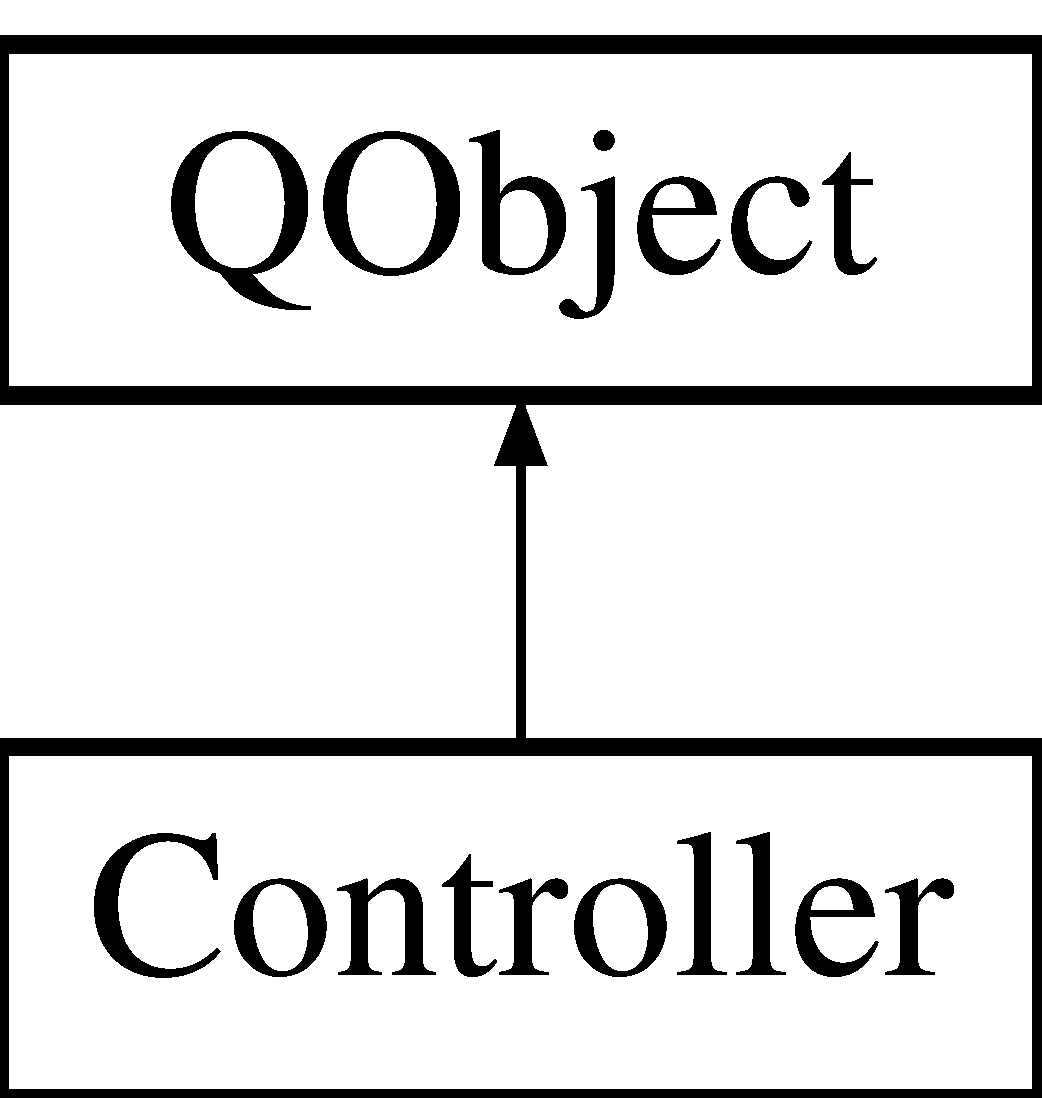
\includegraphics[height=2.000000cm]{class_controller}
\end{center}
\end{figure}
\subsection*{Public Member Functions}
\begin{DoxyCompactItemize}
\item 
\mbox{\hyperlink{class_controller_a2911be3c6cf58c8525aa63d804488b6a}{Controller}} (Q\+Tab\+Widget $\ast$\+\_\+tab\+\_\+widget, Q\+Object $\ast$parent=nullptr)
\begin{DoxyCompactList}\small\item\em Конструктор класса \mbox{\hyperlink{class_controller}{Controller}}. \end{DoxyCompactList}\item 
\mbox{\Hypertarget{class_controller_a0ab87934c4f7a266cfdb86e0f36bc1b5}\label{class_controller_a0ab87934c4f7a266cfdb86e0f36bc1b5}} 
\mbox{\hyperlink{class_controller_a0ab87934c4f7a266cfdb86e0f36bc1b5}{$\sim$\+Controller}} ()
\begin{DoxyCompactList}\small\item\em Деструктор класса \mbox{\hyperlink{class_controller}{Controller}}. \end{DoxyCompactList}\item 
void \mbox{\hyperlink{class_controller_ae788a9a67cbce41929031afcda137b6a}{set\+\_\+working\+\_\+directory}} (const Q\+String \&work\+\_\+dir)
\begin{DoxyCompactList}\small\item\em Задаёт папку для автоматического сохранения C\+SV и DB файлов. \end{DoxyCompactList}\item 
bool \mbox{\hyperlink{class_controller_ada26f78fcec6b246700604b412622d7c}{read\+\_\+csv}} (const Q\+String\+List \&file\+\_\+names)
\begin{DoxyCompactList}\small\item\em Читает таблицы из нескольких файлов C\+SV. В случае неудачи всё очищается и появляется сообщение о неудачном чтении файлов \end{DoxyCompactList}\item 
bool \mbox{\hyperlink{class_controller_ae69865387ccd62da77649c705785c2bc}{read\+\_\+db}} (const Q\+String \&db\+\_\+name)
\begin{DoxyCompactList}\small\item\em Читает все таблицы из базы данных \end{DoxyCompactList}\item 
bool \mbox{\hyperlink{class_controller_a07bd206b7ca5fec8c3a6fb093ed9b307}{convert\+\_\+to\+\_\+csv}} (const Q\+String\+List \&selected\+\_\+names) const
\begin{DoxyCompactList}\small\item\em Преобразует хранящиеся таблицы в несколько файлов C\+SV Преобразуются только выбранные пользователем таблицы \end{DoxyCompactList}\item 
bool \mbox{\hyperlink{class_controller_a1a767cfe7fa199f78b3043f4cd637c76}{convert\+\_\+to\+\_\+db}} (const Q\+String\+List \&selected\+\_\+names) const
\begin{DoxyCompactList}\small\item\em Преобразует хранящиеся таблицы в таблицы базы данных Преобразуются только выбранные пользователем таблицы \end{DoxyCompactList}\item 
Q\+String\+List \mbox{\hyperlink{class_controller_af413760ea8c755a4bff82ff5f070ba17}{get\+\_\+all\+\_\+table\+\_\+names}} () const
\begin{DoxyCompactList}\small\item\em Возвращает имена всех хранящихся таблиц \end{DoxyCompactList}\item 
\mbox{\Hypertarget{class_controller_ab5515748f1b0c82f015e039c817ee5f7}\label{class_controller_ab5515748f1b0c82f015e039c817ee5f7}} 
void \mbox{\hyperlink{class_controller_ab5515748f1b0c82f015e039c817ee5f7}{reset}} ()
\begin{DoxyCompactList}\small\item\em Очищает контроллер \end{DoxyCompactList}\end{DoxyCompactItemize}
\subsection*{Public Attributes}
\begin{DoxyCompactItemize}
\item 
\mbox{\Hypertarget{class_controller_a16e38246321380621fe90b0a0ece1ef4}\label{class_controller_a16e38246321380621fe90b0a0ece1ef4}} 
bool {\bfseries data\+\_\+was\+\_\+load}
\end{DoxyCompactItemize}


\subsection{Detailed Description}
Обеспечивает загрузку данных из файлов в формате C\+SV и DB и выгрузку данных в них. 

\subsection{Constructor \& Destructor Documentation}
\mbox{\Hypertarget{class_controller_a2911be3c6cf58c8525aa63d804488b6a}\label{class_controller_a2911be3c6cf58c8525aa63d804488b6a}} 
\index{Controller@{Controller}!Controller@{Controller}}
\index{Controller@{Controller}!Controller@{Controller}}
\subsubsection{\texorpdfstring{Controller()}{Controller()}}
{\footnotesize\ttfamily Controller\+::\+Controller (\begin{DoxyParamCaption}\item[{Q\+Tab\+Widget $\ast$}]{\+\_\+tab\+\_\+widget,  }\item[{Q\+Object $\ast$}]{parent = {\ttfamily nullptr} }\end{DoxyParamCaption})\hspace{0.3cm}{\ttfamily [explicit]}}



Конструктор класса \mbox{\hyperlink{class_controller}{Controller}}. 


\begin{DoxyParams}{Parameters}
{\em \+\_\+tab\+\_\+widget} & указатель на виджет вывода таблиц \\
\hline
{\em parent} & родительский объект \\
\hline
\end{DoxyParams}


\subsection{Member Function Documentation}
\mbox{\Hypertarget{class_controller_a07bd206b7ca5fec8c3a6fb093ed9b307}\label{class_controller_a07bd206b7ca5fec8c3a6fb093ed9b307}} 
\index{Controller@{Controller}!convert\+\_\+to\+\_\+csv@{convert\+\_\+to\+\_\+csv}}
\index{convert\+\_\+to\+\_\+csv@{convert\+\_\+to\+\_\+csv}!Controller@{Controller}}
\subsubsection{\texorpdfstring{convert\+\_\+to\+\_\+csv()}{convert\_to\_csv()}}
{\footnotesize\ttfamily bool Controller\+::convert\+\_\+to\+\_\+csv (\begin{DoxyParamCaption}\item[{const Q\+String\+List \&}]{selected\+\_\+names }\end{DoxyParamCaption}) const}



Преобразует хранящиеся таблицы в несколько файлов C\+SV Преобразуются только выбранные пользователем таблицы 


\begin{DoxyParams}{Parameters}
{\em selected\+\_\+names} & выбранные таблицы \\
\hline
\end{DoxyParams}
\begin{DoxyReturn}{Returns}
Успешность выполнения функции 
\end{DoxyReturn}
\mbox{\Hypertarget{class_controller_a1a767cfe7fa199f78b3043f4cd637c76}\label{class_controller_a1a767cfe7fa199f78b3043f4cd637c76}} 
\index{Controller@{Controller}!convert\+\_\+to\+\_\+db@{convert\+\_\+to\+\_\+db}}
\index{convert\+\_\+to\+\_\+db@{convert\+\_\+to\+\_\+db}!Controller@{Controller}}
\subsubsection{\texorpdfstring{convert\+\_\+to\+\_\+db()}{convert\_to\_db()}}
{\footnotesize\ttfamily bool Controller\+::convert\+\_\+to\+\_\+db (\begin{DoxyParamCaption}\item[{const Q\+String\+List \&}]{selected\+\_\+names }\end{DoxyParamCaption}) const}



Преобразует хранящиеся таблицы в таблицы базы данных Преобразуются только выбранные пользователем таблицы 


\begin{DoxyParams}{Parameters}
{\em selected\+\_\+names} & выбранные таблицы \\
\hline
\end{DoxyParams}
\begin{DoxyReturn}{Returns}
Успешность выполнения функции 
\end{DoxyReturn}
\mbox{\Hypertarget{class_controller_af413760ea8c755a4bff82ff5f070ba17}\label{class_controller_af413760ea8c755a4bff82ff5f070ba17}} 
\index{Controller@{Controller}!get\+\_\+all\+\_\+table\+\_\+names@{get\+\_\+all\+\_\+table\+\_\+names}}
\index{get\+\_\+all\+\_\+table\+\_\+names@{get\+\_\+all\+\_\+table\+\_\+names}!Controller@{Controller}}
\subsubsection{\texorpdfstring{get\+\_\+all\+\_\+table\+\_\+names()}{get\_all\_table\_names()}}
{\footnotesize\ttfamily Q\+String\+List Controller\+::get\+\_\+all\+\_\+table\+\_\+names (\begin{DoxyParamCaption}{ }\end{DoxyParamCaption}) const}



Возвращает имена всех хранящихся таблиц 

\begin{DoxyReturn}{Returns}
Список имён таблиц 
\end{DoxyReturn}
\mbox{\Hypertarget{class_controller_ada26f78fcec6b246700604b412622d7c}\label{class_controller_ada26f78fcec6b246700604b412622d7c}} 
\index{Controller@{Controller}!read\+\_\+csv@{read\+\_\+csv}}
\index{read\+\_\+csv@{read\+\_\+csv}!Controller@{Controller}}
\subsubsection{\texorpdfstring{read\+\_\+csv()}{read\_csv()}}
{\footnotesize\ttfamily bool Controller\+::read\+\_\+csv (\begin{DoxyParamCaption}\item[{const Q\+String\+List \&}]{file\+\_\+names }\end{DoxyParamCaption})}



Читает таблицы из нескольких файлов C\+SV. В случае неудачи всё очищается и появляется сообщение о неудачном чтении файлов 


\begin{DoxyParams}{Parameters}
{\em file\+\_\+names} & имена файлов для чтения \\
\hline
\end{DoxyParams}
\begin{DoxyReturn}{Returns}
Успешность выполнения функции 
\end{DoxyReturn}
\mbox{\Hypertarget{class_controller_ae69865387ccd62da77649c705785c2bc}\label{class_controller_ae69865387ccd62da77649c705785c2bc}} 
\index{Controller@{Controller}!read\+\_\+db@{read\+\_\+db}}
\index{read\+\_\+db@{read\+\_\+db}!Controller@{Controller}}
\subsubsection{\texorpdfstring{read\+\_\+db()}{read\_db()}}
{\footnotesize\ttfamily bool Controller\+::read\+\_\+db (\begin{DoxyParamCaption}\item[{const Q\+String \&}]{db\+\_\+name }\end{DoxyParamCaption})}



Читает все таблицы из базы данных 


\begin{DoxyParams}{Parameters}
{\em db\+\_\+name} & имя файла базы данных \\
\hline
\end{DoxyParams}
\begin{DoxyReturn}{Returns}
Успешность выполнения функции 
\end{DoxyReturn}
\mbox{\Hypertarget{class_controller_ae788a9a67cbce41929031afcda137b6a}\label{class_controller_ae788a9a67cbce41929031afcda137b6a}} 
\index{Controller@{Controller}!set\+\_\+working\+\_\+directory@{set\+\_\+working\+\_\+directory}}
\index{set\+\_\+working\+\_\+directory@{set\+\_\+working\+\_\+directory}!Controller@{Controller}}
\subsubsection{\texorpdfstring{set\+\_\+working\+\_\+directory()}{set\_working\_directory()}}
{\footnotesize\ttfamily void Controller\+::set\+\_\+working\+\_\+directory (\begin{DoxyParamCaption}\item[{const Q\+String \&}]{work\+\_\+dir }\end{DoxyParamCaption})}



Задаёт папку для автоматического сохранения C\+SV и DB файлов. 


\begin{DoxyParams}{Parameters}
{\em work\+\_\+dir} & строковое представление папки \\
\hline
\end{DoxyParams}


The documentation for this class was generated from the following files\+:\begin{DoxyCompactItemize}
\item 
Controller.\+h\item 
Controller.\+cpp\end{DoxyCompactItemize}

\hypertarget{class_csv_table_model}{}\section{Csv\+Table\+Model Class Reference}
\label{class_csv_table_model}\index{Csv\+Table\+Model@{Csv\+Table\+Model}}


Класс модели, хранящий в себе данные из C\+S\+V-\/файла  




{\ttfamily \#include $<$Csv\+Table\+Model.\+h$>$}

Inheritance diagram for Csv\+Table\+Model\+:\begin{figure}[H]
\begin{center}
\leavevmode
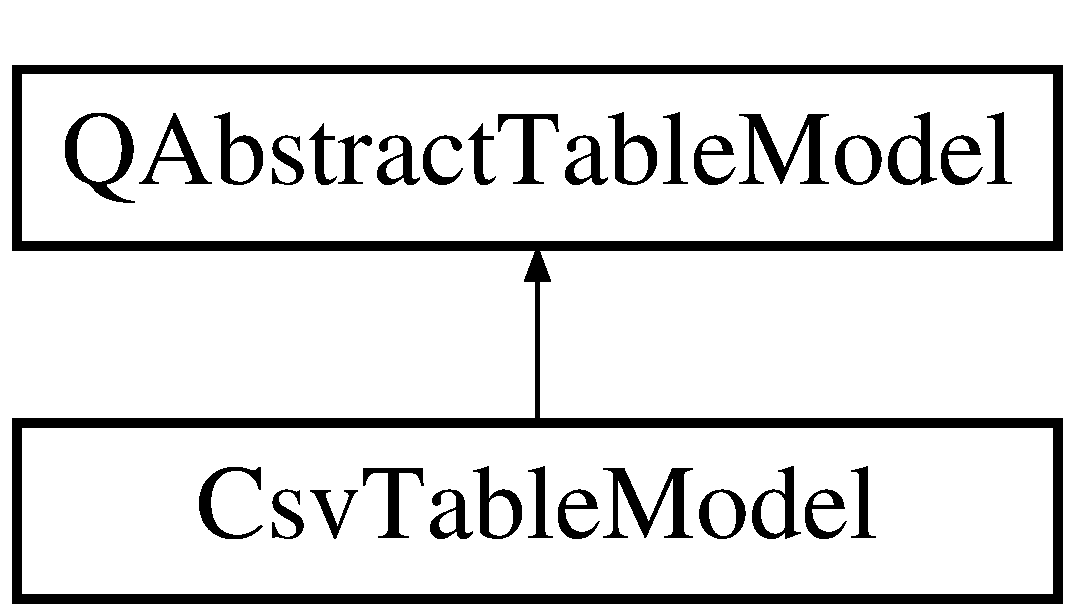
\includegraphics[height=2.000000cm]{class_csv_table_model}
\end{center}
\end{figure}
\subsection*{Public Member Functions}
\begin{DoxyCompactItemize}
\item 
\mbox{\hyperlink{class_csv_table_model_ace3bbe6a48fe262b451dfe5f33577e96}{Csv\+Table\+Model}} (Q\+Object $\ast$parent=nullptr)
\begin{DoxyCompactList}\small\item\em Конструктор \end{DoxyCompactList}\item 
virtual int \mbox{\hyperlink{class_csv_table_model_a91cc21d209c0b9ba8143aa033450bc6e}{row\+Count}} (const Q\+Model\+Index \&parent=Q\+Model\+Index()) const override
\begin{DoxyCompactList}\small\item\em Возвращает количество строк в таблице \end{DoxyCompactList}\item 
virtual int \mbox{\hyperlink{class_csv_table_model_a750aedb5638fc8e04e9a6e530a119f91}{column\+Count}} (const Q\+Model\+Index \&parent=Q\+Model\+Index()) const override
\begin{DoxyCompactList}\small\item\em Возвращает количество столбцов таблицы \end{DoxyCompactList}\item 
virtual Q\+Variant \mbox{\hyperlink{class_csv_table_model_a86cfc5e15808768e3517f5183e7d5fbb}{data}} (const Q\+Model\+Index \&index, int role) const override
\begin{DoxyCompactList}\small\item\em Возвращает данные, хранящиеся по указанному индексу \end{DoxyCompactList}\item 
virtual Q\+Variant \mbox{\hyperlink{class_csv_table_model_ae5790a6d1cbfcfdf7b8b5a4ce4a63748}{header\+Data}} (int section, Qt\+::\+Orientation orientation, int role) const override
\begin{DoxyCompactList}\small\item\em Возвращает имя выбранного столбца таблицы \end{DoxyCompactList}\item 
\mbox{\Hypertarget{class_csv_table_model_a24f940138776feeed8d5884731a2cea4}\label{class_csv_table_model_a24f940138776feeed8d5884731a2cea4}} 
void \mbox{\hyperlink{class_csv_table_model_a24f940138776feeed8d5884731a2cea4}{reset}} ()
\begin{DoxyCompactList}\small\item\em Очищает модель \end{DoxyCompactList}\item 
bool \mbox{\hyperlink{class_csv_table_model_a05af2e7652238643f3f54c964eec2ec2}{read}} (const Q\+String \&file\+\_\+name)
\begin{DoxyCompactList}\small\item\em Чтение таблицы из файла \end{DoxyCompactList}\end{DoxyCompactItemize}


\subsection{Detailed Description}
Класс модели, хранящий в себе данные из C\+S\+V-\/файла 

\subsection{Constructor \& Destructor Documentation}
\mbox{\Hypertarget{class_csv_table_model_ace3bbe6a48fe262b451dfe5f33577e96}\label{class_csv_table_model_ace3bbe6a48fe262b451dfe5f33577e96}} 
\index{Csv\+Table\+Model@{Csv\+Table\+Model}!Csv\+Table\+Model@{Csv\+Table\+Model}}
\index{Csv\+Table\+Model@{Csv\+Table\+Model}!Csv\+Table\+Model@{Csv\+Table\+Model}}
\subsubsection{\texorpdfstring{Csv\+Table\+Model()}{CsvTableModel()}}
{\footnotesize\ttfamily Csv\+Table\+Model\+::\+Csv\+Table\+Model (\begin{DoxyParamCaption}\item[{Q\+Object $\ast$}]{parent = {\ttfamily nullptr} }\end{DoxyParamCaption})\hspace{0.3cm}{\ttfamily [inline]}, {\ttfamily [explicit]}}



Конструктор 


\begin{DoxyParams}{Parameters}
{\em parent} & родитель \\
\hline
\end{DoxyParams}


\subsection{Member Function Documentation}
\mbox{\Hypertarget{class_csv_table_model_a750aedb5638fc8e04e9a6e530a119f91}\label{class_csv_table_model_a750aedb5638fc8e04e9a6e530a119f91}} 
\index{Csv\+Table\+Model@{Csv\+Table\+Model}!column\+Count@{column\+Count}}
\index{column\+Count@{column\+Count}!Csv\+Table\+Model@{Csv\+Table\+Model}}
\subsubsection{\texorpdfstring{column\+Count()}{columnCount()}}
{\footnotesize\ttfamily int Csv\+Table\+Model\+::column\+Count (\begin{DoxyParamCaption}\item[{const Q\+Model\+Index \&}]{parent = {\ttfamily QModelIndex()} }\end{DoxyParamCaption}) const\hspace{0.3cm}{\ttfamily [override]}, {\ttfamily [virtual]}}



Возвращает количество столбцов таблицы 


\begin{DoxyParams}{Parameters}
{\em parent} & родитель \\
\hline
\end{DoxyParams}
\begin{DoxyReturn}{Returns}
Количество строк 
\end{DoxyReturn}
\mbox{\Hypertarget{class_csv_table_model_a86cfc5e15808768e3517f5183e7d5fbb}\label{class_csv_table_model_a86cfc5e15808768e3517f5183e7d5fbb}} 
\index{Csv\+Table\+Model@{Csv\+Table\+Model}!data@{data}}
\index{data@{data}!Csv\+Table\+Model@{Csv\+Table\+Model}}
\subsubsection{\texorpdfstring{data()}{data()}}
{\footnotesize\ttfamily Q\+Variant Csv\+Table\+Model\+::data (\begin{DoxyParamCaption}\item[{const Q\+Model\+Index \&}]{index,  }\item[{int}]{role }\end{DoxyParamCaption}) const\hspace{0.3cm}{\ttfamily [override]}, {\ttfamily [virtual]}}



Возвращает данные, хранящиеся по указанному индексу 


\begin{DoxyParams}{Parameters}
{\em index} & индекс \\
\hline
{\em role} & роль \\
\hline
\end{DoxyParams}
\begin{DoxyReturn}{Returns}
Данные, хранящиеся по индексу 
\end{DoxyReturn}
\mbox{\Hypertarget{class_csv_table_model_ae5790a6d1cbfcfdf7b8b5a4ce4a63748}\label{class_csv_table_model_ae5790a6d1cbfcfdf7b8b5a4ce4a63748}} 
\index{Csv\+Table\+Model@{Csv\+Table\+Model}!header\+Data@{header\+Data}}
\index{header\+Data@{header\+Data}!Csv\+Table\+Model@{Csv\+Table\+Model}}
\subsubsection{\texorpdfstring{header\+Data()}{headerData()}}
{\footnotesize\ttfamily Q\+Variant Csv\+Table\+Model\+::header\+Data (\begin{DoxyParamCaption}\item[{int}]{section,  }\item[{Qt\+::\+Orientation}]{orientation,  }\item[{int}]{role }\end{DoxyParamCaption}) const\hspace{0.3cm}{\ttfamily [override]}, {\ttfamily [virtual]}}



Возвращает имя выбранного столбца таблицы 


\begin{DoxyParams}{Parameters}
{\em section} & номер столбца \\
\hline
{\em orientation} & ориентация \\
\hline
{\em role} & роль \\
\hline
\end{DoxyParams}
\begin{DoxyReturn}{Returns}
Имя столбца 
\end{DoxyReturn}
\mbox{\Hypertarget{class_csv_table_model_a05af2e7652238643f3f54c964eec2ec2}\label{class_csv_table_model_a05af2e7652238643f3f54c964eec2ec2}} 
\index{Csv\+Table\+Model@{Csv\+Table\+Model}!read@{read}}
\index{read@{read}!Csv\+Table\+Model@{Csv\+Table\+Model}}
\subsubsection{\texorpdfstring{read()}{read()}}
{\footnotesize\ttfamily bool Csv\+Table\+Model\+::read (\begin{DoxyParamCaption}\item[{const Q\+String \&}]{file\+\_\+name }\end{DoxyParamCaption})}



Чтение таблицы из файла 


\begin{DoxyParams}{Parameters}
{\em file\+\_\+name} & имя входного файла \\
\hline
\end{DoxyParams}
\begin{DoxyReturn}{Returns}
Успешность выполнения операции 
\end{DoxyReturn}
\mbox{\Hypertarget{class_csv_table_model_a91cc21d209c0b9ba8143aa033450bc6e}\label{class_csv_table_model_a91cc21d209c0b9ba8143aa033450bc6e}} 
\index{Csv\+Table\+Model@{Csv\+Table\+Model}!row\+Count@{row\+Count}}
\index{row\+Count@{row\+Count}!Csv\+Table\+Model@{Csv\+Table\+Model}}
\subsubsection{\texorpdfstring{row\+Count()}{rowCount()}}
{\footnotesize\ttfamily int Csv\+Table\+Model\+::row\+Count (\begin{DoxyParamCaption}\item[{const Q\+Model\+Index \&}]{parent = {\ttfamily QModelIndex()} }\end{DoxyParamCaption}) const\hspace{0.3cm}{\ttfamily [override]}, {\ttfamily [virtual]}}



Возвращает количество строк в таблице 


\begin{DoxyParams}{Parameters}
{\em parent} & родитель \\
\hline
\end{DoxyParams}
\begin{DoxyReturn}{Returns}
Количество строк 
\end{DoxyReturn}


The documentation for this class was generated from the following files\+:\begin{DoxyCompactItemize}
\item 
Csv\+Table\+Model.\+h\item 
Csv\+Table\+Model.\+cpp\end{DoxyCompactItemize}

\hypertarget{class_main_window}{}\section{Main\+Window Class Reference}
\label{class_main_window}\index{Main\+Window@{Main\+Window}}


Главное окно приложения  




{\ttfamily \#include $<$mainwindow.\+h$>$}

Inheritance diagram for Main\+Window\+:\begin{figure}[H]
\begin{center}
\leavevmode
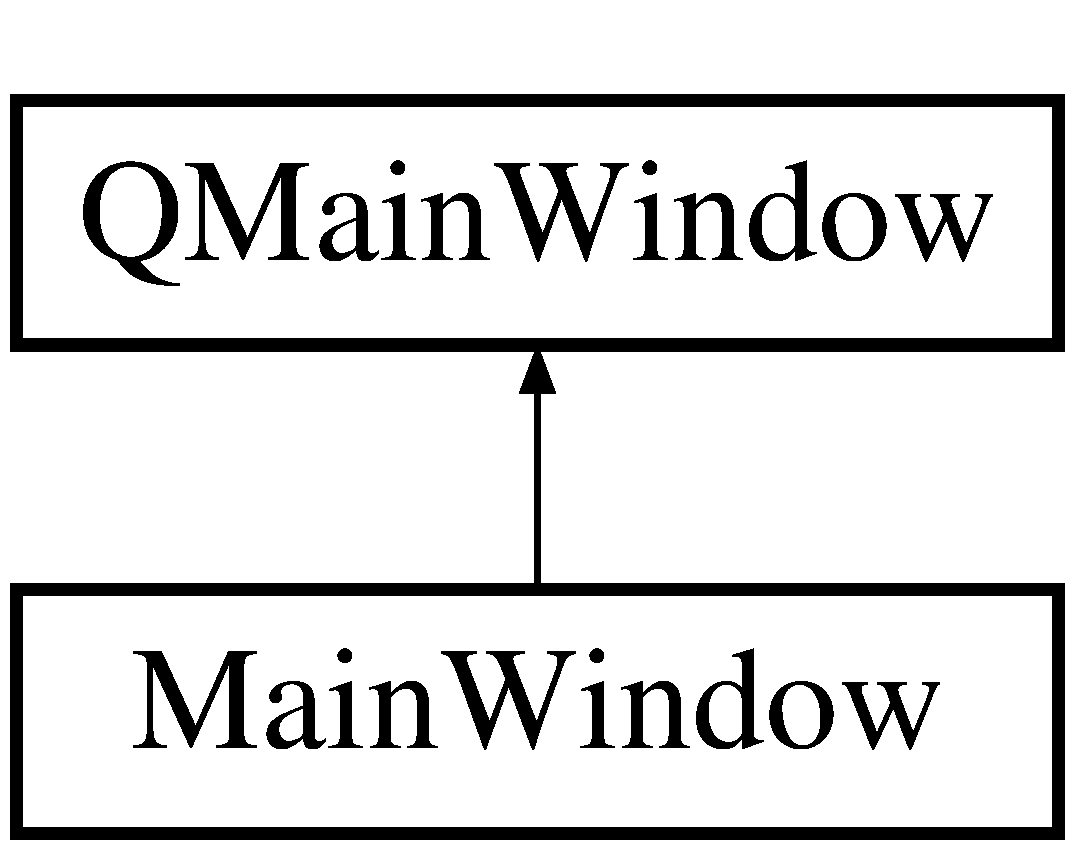
\includegraphics[height=2.000000cm]{class_main_window}
\end{center}
\end{figure}
\subsection*{Public Member Functions}
\begin{DoxyCompactItemize}
\item 
\mbox{\hyperlink{class_main_window_a8b244be8b7b7db1b08de2a2acb9409db}{Main\+Window}} (Q\+Widget $\ast$parent=0)
\begin{DoxyCompactList}\small\item\em Конструктор \end{DoxyCompactList}\item 
\mbox{\Hypertarget{class_main_window_ae98d00a93bc118200eeef9f9bba1dba7}\label{class_main_window_ae98d00a93bc118200eeef9f9bba1dba7}} 
\mbox{\hyperlink{class_main_window_ae98d00a93bc118200eeef9f9bba1dba7}{$\sim$\+Main\+Window}} ()
\begin{DoxyCompactList}\small\item\em Деструктор класса \mbox{\hyperlink{class_main_window}{Main\+Window}}. \end{DoxyCompactList}\end{DoxyCompactItemize}


\subsection{Detailed Description}
Главное окно приложения 

\subsection{Constructor \& Destructor Documentation}
\mbox{\Hypertarget{class_main_window_a8b244be8b7b7db1b08de2a2acb9409db}\label{class_main_window_a8b244be8b7b7db1b08de2a2acb9409db}} 
\index{Main\+Window@{Main\+Window}!Main\+Window@{Main\+Window}}
\index{Main\+Window@{Main\+Window}!Main\+Window@{Main\+Window}}
\subsubsection{\texorpdfstring{Main\+Window()}{MainWindow()}}
{\footnotesize\ttfamily Main\+Window\+::\+Main\+Window (\begin{DoxyParamCaption}\item[{Q\+Widget $\ast$}]{parent = {\ttfamily 0} }\end{DoxyParamCaption})\hspace{0.3cm}{\ttfamily [explicit]}}



Конструктор 


\begin{DoxyParams}{Parameters}
{\em parent} & родитель \\
\hline
\end{DoxyParams}


The documentation for this class was generated from the following files\+:\begin{DoxyCompactItemize}
\item 
mainwindow.\+h\item 
mainwindow.\+cpp\end{DoxyCompactItemize}

\hypertarget{class_select_names_dialog}{}\section{Select\+Names\+Dialog Class Reference}
\label{class_select_names_dialog}\index{Select\+Names\+Dialog@{Select\+Names\+Dialog}}


Класс выбора имён таблиц для выгрузки в C\+SV или DB.  




{\ttfamily \#include $<$Select\+Names\+Dialog.\+h$>$}

Inheritance diagram for Select\+Names\+Dialog\+:\begin{figure}[H]
\begin{center}
\leavevmode
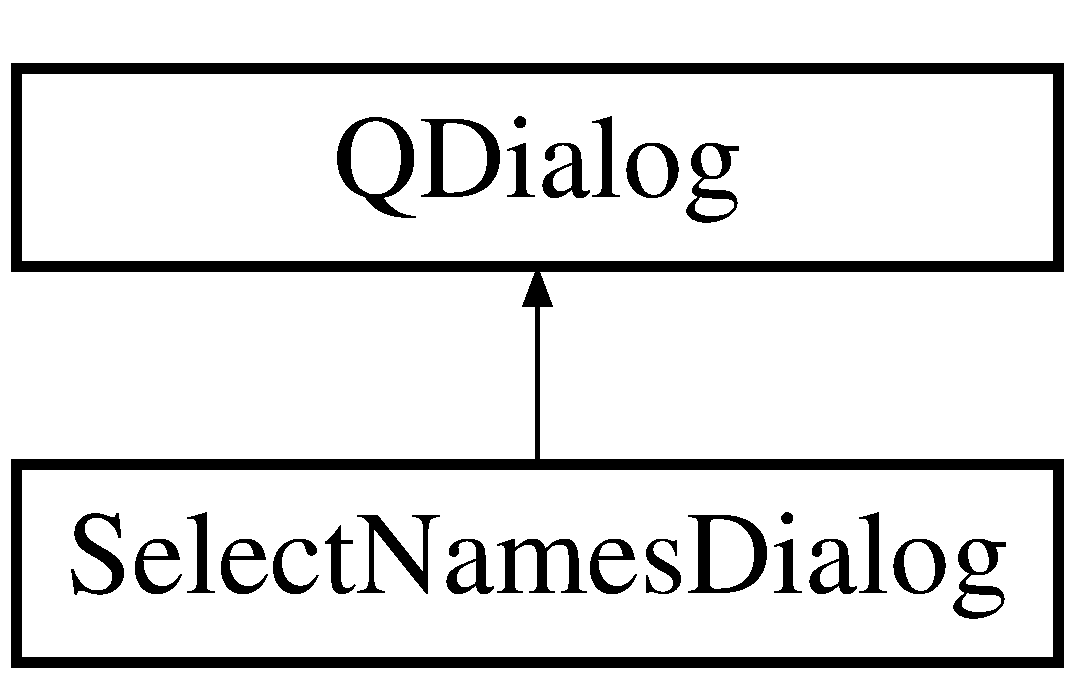
\includegraphics[height=2.000000cm]{class_select_names_dialog}
\end{center}
\end{figure}
\subsection*{Public Member Functions}
\begin{DoxyCompactItemize}
\item 
\mbox{\hyperlink{class_select_names_dialog_af5d6957152caad6629fe390127f8fe90}{Select\+Names\+Dialog}} (const Q\+String\+List \&names, Q\+Widget $\ast$parent=0)
\begin{DoxyCompactList}\small\item\em Конструктор \end{DoxyCompactList}\item 
\mbox{\Hypertarget{class_select_names_dialog_a054490a68f2182d983ec7c68eb1ef873}\label{class_select_names_dialog_a054490a68f2182d983ec7c68eb1ef873}} 
\mbox{\hyperlink{class_select_names_dialog_a054490a68f2182d983ec7c68eb1ef873}{$\sim$\+Select\+Names\+Dialog}} ()
\begin{DoxyCompactList}\small\item\em Деструктор \end{DoxyCompactList}\item 
Q\+String\+List \mbox{\hyperlink{class_select_names_dialog_a063b06a2ee6f46d0aa2ae5399d18ff04}{get\+\_\+selected\+\_\+names}} ()
\begin{DoxyCompactList}\small\item\em Вызывает диалоговое окно, ожидает выбор пользователя и возвращает выбранные им имена таблиц \end{DoxyCompactList}\end{DoxyCompactItemize}


\subsection{Detailed Description}
Класс выбора имён таблиц для выгрузки в C\+SV или DB. 

\subsection{Constructor \& Destructor Documentation}
\mbox{\Hypertarget{class_select_names_dialog_af5d6957152caad6629fe390127f8fe90}\label{class_select_names_dialog_af5d6957152caad6629fe390127f8fe90}} 
\index{Select\+Names\+Dialog@{Select\+Names\+Dialog}!Select\+Names\+Dialog@{Select\+Names\+Dialog}}
\index{Select\+Names\+Dialog@{Select\+Names\+Dialog}!Select\+Names\+Dialog@{Select\+Names\+Dialog}}
\subsubsection{\texorpdfstring{Select\+Names\+Dialog()}{SelectNamesDialog()}}
{\footnotesize\ttfamily Select\+Names\+Dialog\+::\+Select\+Names\+Dialog (\begin{DoxyParamCaption}\item[{const Q\+String\+List \&}]{names,  }\item[{Q\+Widget $\ast$}]{parent = {\ttfamily 0} }\end{DoxyParamCaption})\hspace{0.3cm}{\ttfamily [explicit]}}



Конструктор 


\begin{DoxyParams}{Parameters}
{\em names} & все имена таблиц, из которых пользователь должен выбрать нужные \\
\hline
{\em parent} & родитель \\
\hline
\end{DoxyParams}


\subsection{Member Function Documentation}
\mbox{\Hypertarget{class_select_names_dialog_a063b06a2ee6f46d0aa2ae5399d18ff04}\label{class_select_names_dialog_a063b06a2ee6f46d0aa2ae5399d18ff04}} 
\index{Select\+Names\+Dialog@{Select\+Names\+Dialog}!get\+\_\+selected\+\_\+names@{get\+\_\+selected\+\_\+names}}
\index{get\+\_\+selected\+\_\+names@{get\+\_\+selected\+\_\+names}!Select\+Names\+Dialog@{Select\+Names\+Dialog}}
\subsubsection{\texorpdfstring{get\+\_\+selected\+\_\+names()}{get\_selected\_names()}}
{\footnotesize\ttfamily Q\+String\+List Select\+Names\+Dialog\+::get\+\_\+selected\+\_\+names (\begin{DoxyParamCaption}{ }\end{DoxyParamCaption})}



Вызывает диалоговое окно, ожидает выбор пользователя и возвращает выбранные им имена таблиц 

\begin{DoxyReturn}{Returns}
Выбранные имена таблиц 
\end{DoxyReturn}


The documentation for this class was generated from the following files\+:\begin{DoxyCompactItemize}
\item 
Select\+Names\+Dialog.\+h\item 
Select\+Names\+Dialog.\+cpp\end{DoxyCompactItemize}

%--- End generated contents ---

% Index
\backmatter
\newpage
\phantomsection
\clearemptydoublepage
\addcontentsline{toc}{chapter}{Index}
\printindex

\end{document}
